\chapter{Pictures}

\begin{table}[ht]
    \centering
    \begin{tabular}{c}
    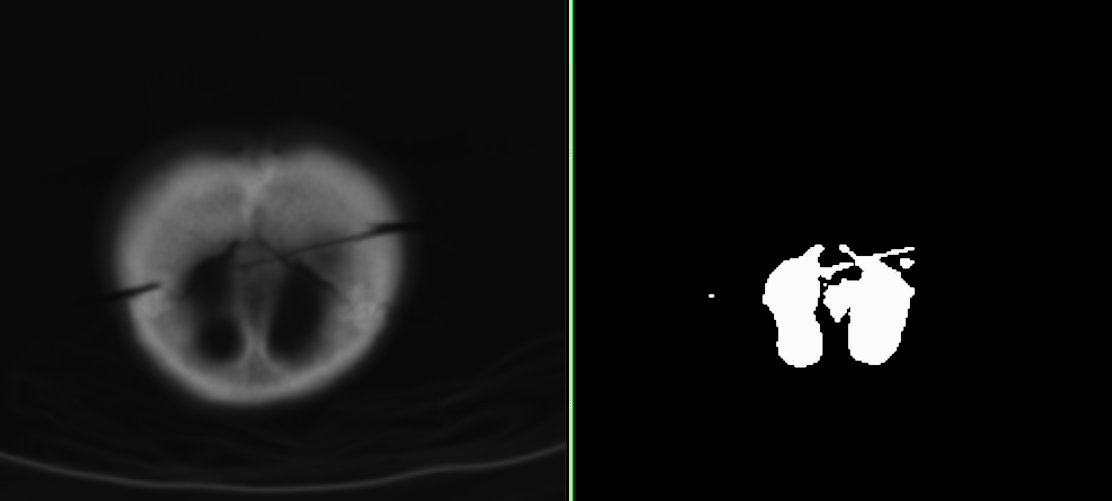
\includegraphics[scale=.5]{data/png/2}\\
    \newline
    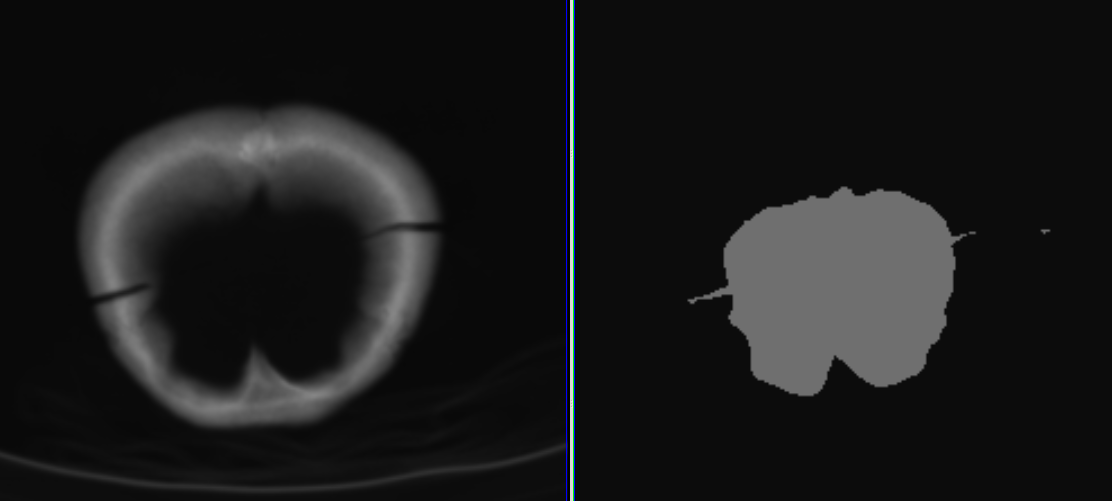
\includegraphics[scale=.5]{data/png/4}\\
    \newline
    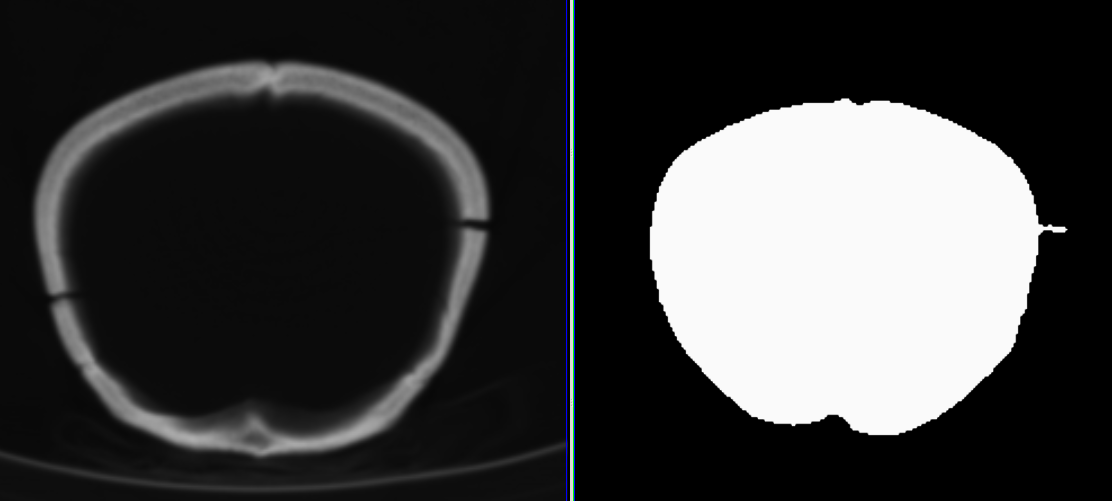
\includegraphics[scale=.5]{data/png/7}\\
    \newline
    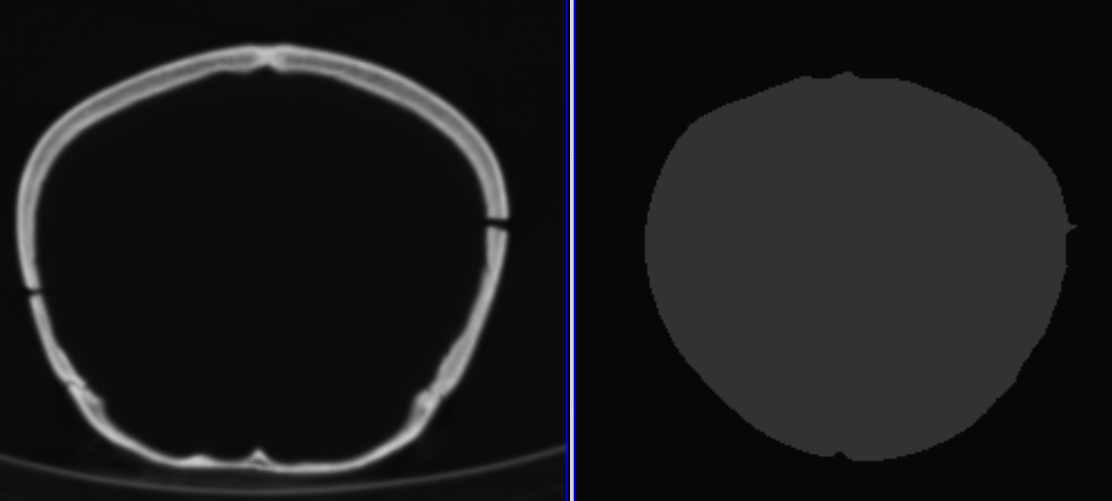
\includegraphics[scale=.5]{data/png/12}\\
    \end{tabular}
    \label{tab:gt1}
\end{table}%

\begin{table}[ht]
    \centering
    \begin{tabular}{c}
    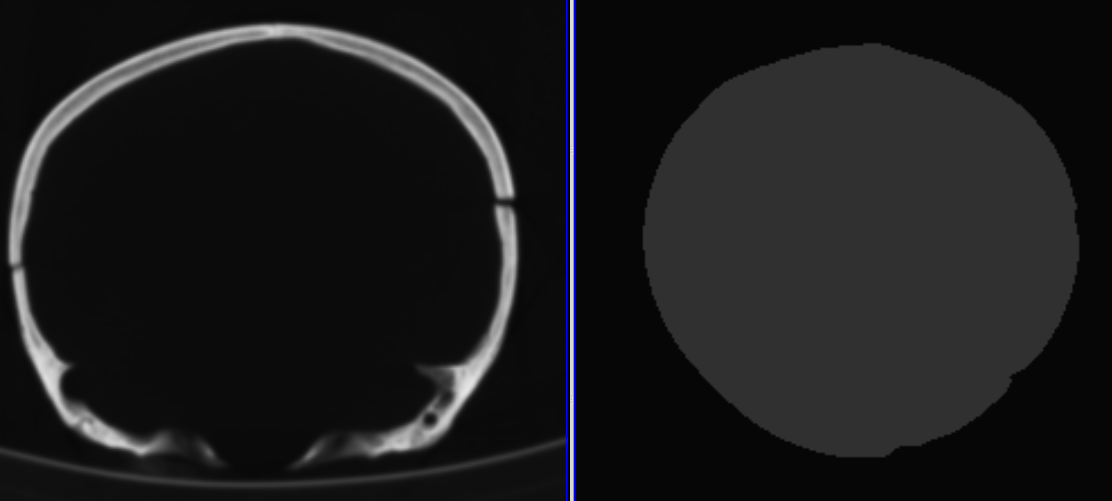
\includegraphics[scale=.5]{data/png/15}\\
    \newline
    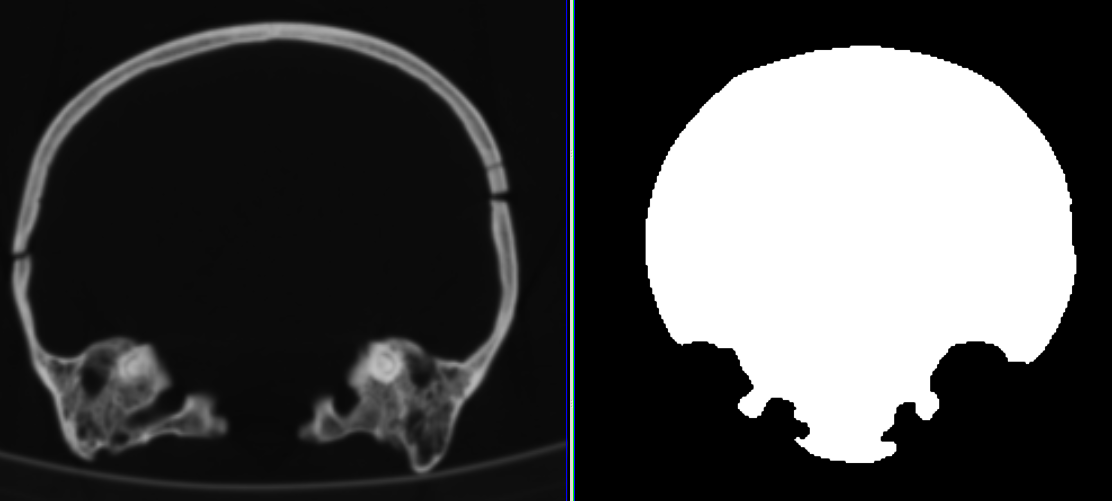
\includegraphics[scale=.5]{data/png/17}\\
    \newline
    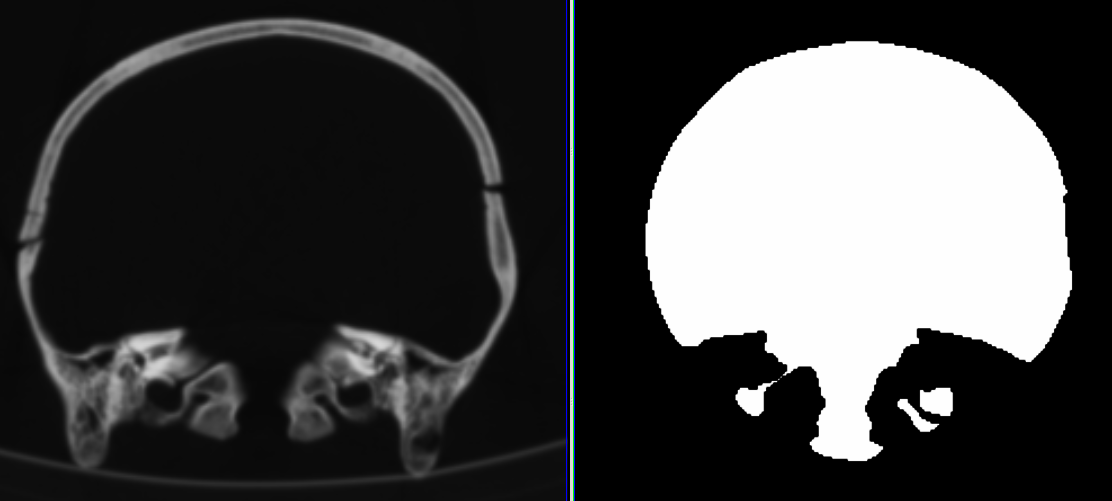
\includegraphics[scale=.5]{data/png/18}\\
    \newline
    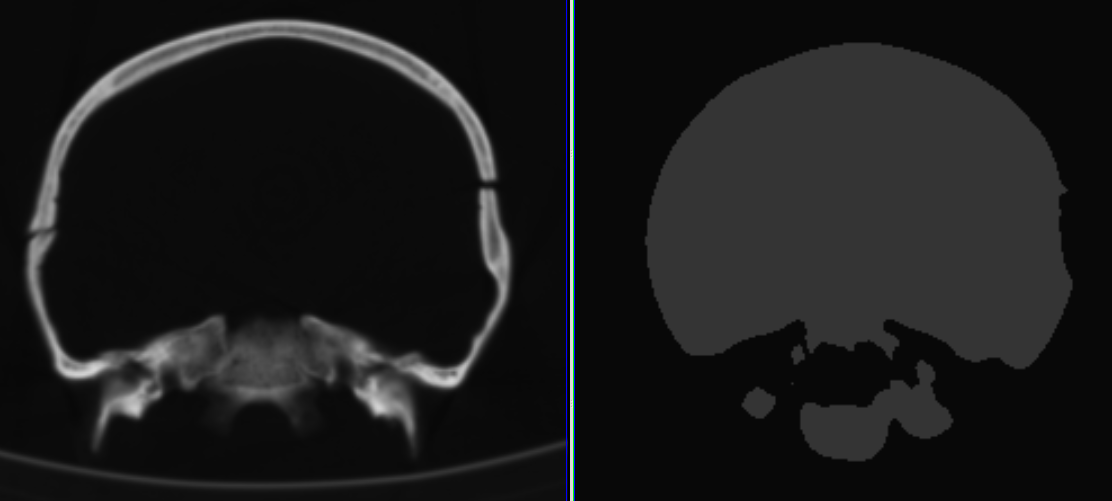
\includegraphics[scale=.5]{data/png/19}\\
    \end{tabular}
    \label{tab:gt2}
\end{table}%

\begin{table}[ht]
    \centering
    \begin{tabular}{c}
    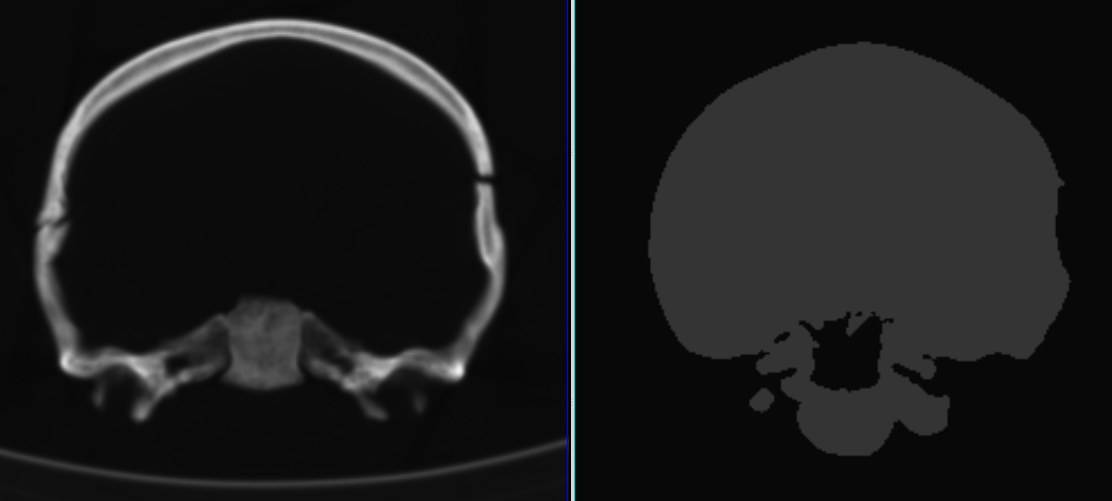
\includegraphics[scale=.5]{data/png/20}\\
    \newline
    
\includegraphics[scale=.5]{data/png/23}\\
    \newline
    
\includegraphics[scale=.5]{data/png/25}\\
    \newline
    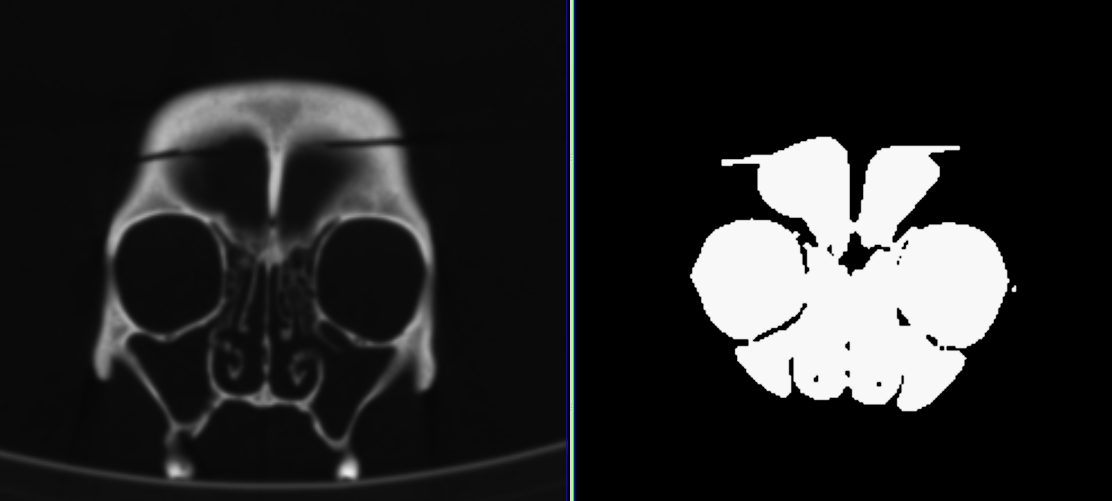
\includegraphics[scale=.5]{data/png/27}\\
    \end{tabular}
    \label{tab:gt3}
\end{table}%

\begin{table}[ht]
    \centering
    \begin{tabular}{c}
    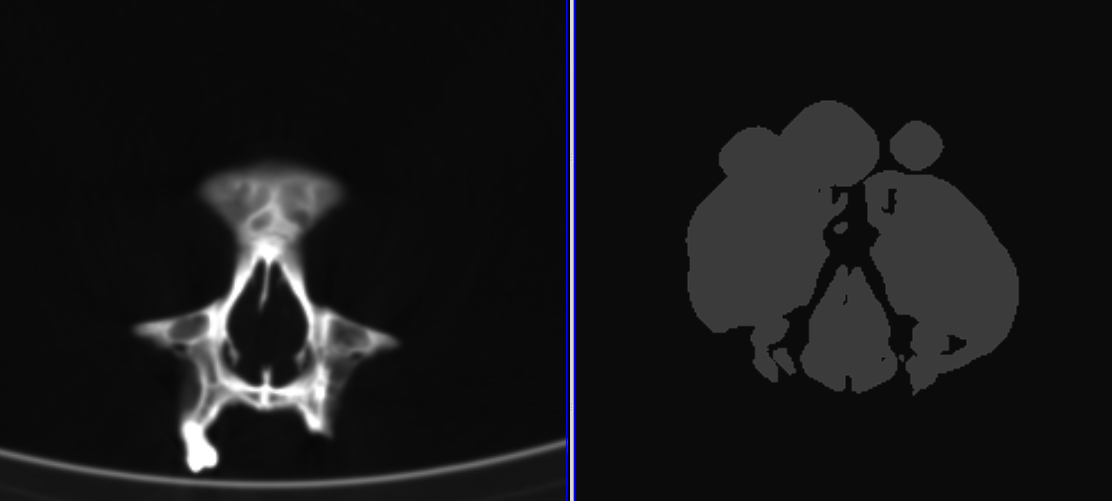
\includegraphics[scale=.5]{data/png/29}\\
    \newline
    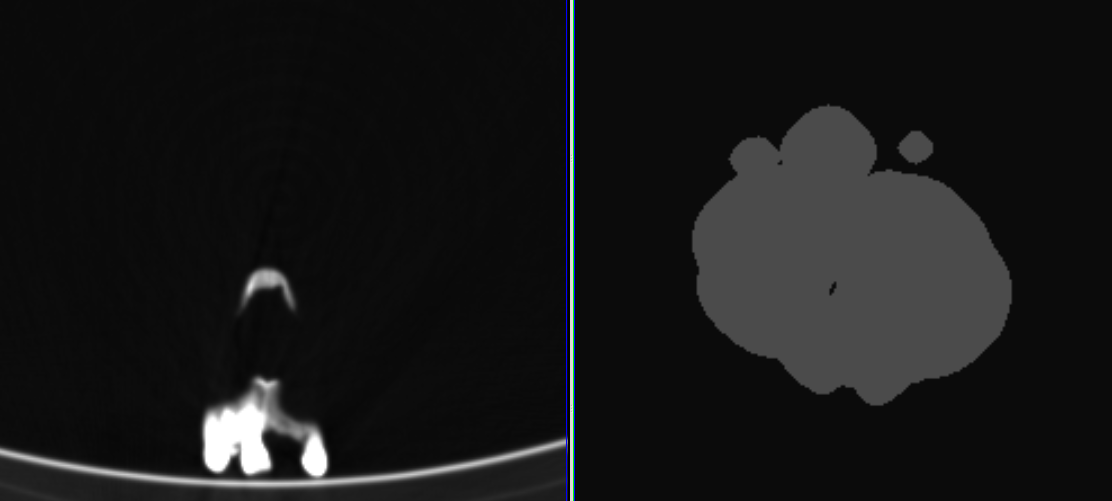
\includegraphics[scale=.5]{data/png/31}\\
    \end{tabular}
    \caption[Segmented data set]
{
Images of slices of segmented data set. Original data set (on the left) and segmented one (on the right).
}
\end{table}%


\begin{figure}[h]
    \centering
    
\includegraphics[width=0.6\textwidth]{data/png/3d}
    \caption[Series3DView]
{
3D View of segmented data set. VTK viewer used to visualize the data set.
}
    \label{fg:series3d}
\end{figure}